\documentclass[12pt,b5paper]{ltjsarticle}

%\usepackage[margin=15truemm, top=5truemm, bottom=5truemm]{geometry}
%\usepackage[margin=10truemm,left=15truemm]{geometry}
\usepackage[margin=10truemm]{geometry}

\usepackage{amsmath,amssymb}
%\pagestyle{headings}
\pagestyle{empty}

%\usepackage{listings,url}
\renewcommand{\theenumi}{(\arabic{enumi})}


%\usepackage{graphicx}

\usepackage{tikz} % draw graphics : TikZ ist kein Zeichenprogramm
\usetikzlibrary{arrows.meta}

%\usepackage{wrapfig}
%\usepackage{bm} % ベクトルの矢印

%\usepackage{luatexja-ruby} % ルビを振る

%% 核Ker 像Im Hom を定義
%\newcommand{\Img}{\mathop{\mathrm{Im}}\nolimits}
%\newcommand{\Ker}{\mathop{\mathrm{Ker}}\nolimits}
%\newcommand{\Hom}{\mathop{\mathrm{Hom}}\nolimits}

%\DeclareMathOperator{\Rot}{rot}
%\DeclareMathOperator{\Div}{div}
%\DeclareMathOperator{\Grad}{grad}
%\DeclareMathOperator{\arcsinh}{arcsinh}
%\DeclareMathOperator{\arccosh}{arccosh}
%\DeclareMathOperator{\arctanh}{arctanh}

\usepackage{url} % URLの記述

%\usepackage{listings}
%
%\lstset{
%%プログラム言語(複数の言語に対応,C,C++も可)
%  language = Python,
%%  language = Lisp,
%%  language = C,
%  %背景色と透過度
%  %backgroundcolor={\color[gray]{.90}},
%  %枠外に行った時の自動改行
%  breaklines = true,
%  %自動改行後のインデント量(デフォルトでは20[pt])
%  breakindent = 10pt,
%  %標準の書体
%%  basicstyle = \ttfamily\scriptsize,
%  basicstyle = \ttfamily,
%  %コメントの書体
%%  commentstyle = {\itshape \color[cmyk]{1,0.4,1,0}},
%  %関数名等の色の設定
%  classoffset = 0,
%  %キーワード(int, ifなど)の書体
%%  keywordstyle = {\bfseries \color[cmyk]{0,1,0,0}},
%  %表示する文字の書体
%  %stringstyle = {\ttfamily \color[rgb]{0,0,1}},
%  %枠 "t"は上に線を記載, "T"は上に二重線を記載
%  %他オプション:leftline,topline,bottomline,lines,single,shadowbox
%  frame = TBrl,
%  %frameまでの間隔(行番号とプログラムの間)
%  framesep = 5pt,
%  %行番号の位置
%  numbers = left,
%  %行番号の間隔
%  stepnumber = 1,
%  %行番号の書体
%%  numberstyle = \tiny,
%  %タブの大きさ
%  tabsize = 4,
%  %キャプションの場所("tb"ならば上下両方に記載)
%  captionpos = t
%}

%\usepackage{cancel}
%\usepackage{bussproofs}
%\usepackage{proof}

\begin{document}



\begin{equation}
 \text{3点} \: A,B,C \: \text{が一直線上にある}
  \Leftrightarrow
  {}^{\exists} k\text{:定数}
  \: \mathrm{s.t.} \:
 \overrightarrow{\mathrm{AB}}= k \overrightarrow{\mathrm{AC}}
\end{equation}

\dotfill

線分$AB$を$m:n$に内分する点を$P$とする。
点$A,B$の位置ベクトルを$\vec{a}, \: \vec{b}$とすると、
点$P$の位置ベクトル$\vec{p}$は次を満たす。
\begin{equation}
 \vec{p} = \frac{n \vec{a} + m \vec{b}}{m+n}
\end{equation}



%%%%%%%%%%%%%%%%%%%%%%%%%%%%%%%%%%%%%%%%
\hrulefill

\begin{minipage}[c]{200pt}
$\triangle \mathrm{ABC}$において、
辺$\mathrm{BC}$を$2:1$に外分する点を$\mathrm{P}$、
辺$\mathrm{AB}$を$1:2$に内分する点を$\mathrm{Q}$、
辺$\mathrm{CA}$の中点を$\mathrm{R}$とする。
\begin{enumerate}
 \item 3点$\mathrm{P,\:Q,\:R}$は一直線上にあることを証明せよ。
 \item $\mathrm{QR:QP}$を求めよ。
\end{enumerate}
\end{minipage}
%
\begin{minipage}[c]{200pt}
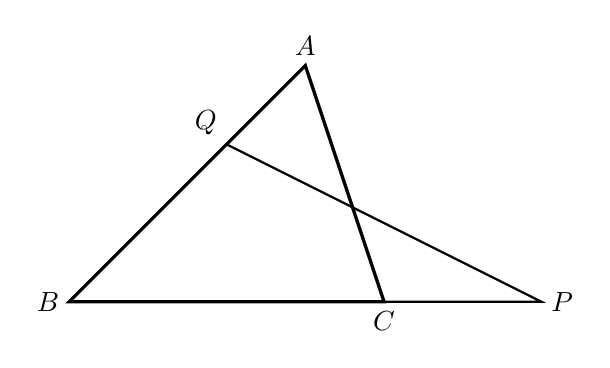
\begin{tikzpicture}[scale=1.0]
 \coordinate (A) at (3,3) node at (A) [above] {$A$}; % A(3,3)を設定,上に$A$
 \coordinate (B) at (0,0) node at (B) [left] {$B$}; % B(0,0)を設定,左に$B$
 \coordinate (C) at (4,0) node at (C) [below] {$C$}; % C(4,0)を設定,下に$C$

 \coordinate (P) at (6,0) node at (P) [right] {$P$}; % P(8,0)を設定,右に$P$
 \coordinate (Q) at (2,2) node at (Q) [above left] {$Q$}; % Q(2,2)を設定,左上に$Q$

 \draw [very thick] (A) -- (B) -- (C) -- cycle;
 \draw [thick] (C) -- (P) -- (Q);
\end{tikzpicture}
\end{minipage}

\dotfill

ベクトル$\vec{b},\:\vec{c}$を
$\vec{b} = \overrightarrow{\mathrm{AB}},\vec{c} = \overrightarrow{\mathrm{AC}}$
とする。

\begin{enumerate}
 \item
      $\overrightarrow{\mathrm{PQ}}$と
      $\overrightarrow{\mathrm{PR}}$を
      $\vec{b},\vec{c}$で表す。

      $P$は$BC$を$2:1$に外分した点であるから
      $\overrightarrow{\mathrm{BP}} = 2\overrightarrow{\mathrm{BC}}$
      である。

      $\overrightarrow{\mathrm{BP}}
      = \overrightarrow{\mathrm{BC}} + \overrightarrow{\mathrm{CP}}$
      であるから、
      $\overrightarrow{\mathrm{CB}} = \overrightarrow{\mathrm{PC}}$
      である。

      $R$は$AC$の中点であるから、
      $\overrightarrow{\mathrm{CR}}=\frac{1}{2}\overrightarrow{\mathrm{CA}}$
      である。

      $\overrightarrow{\mathrm{CA}}=-\vec{c},\:\overrightarrow{\mathrm{CB}} = \vec{b}-\vec{c}$であるから
      $\overrightarrow{\mathrm{PQ}},\:\overrightarrow{\mathrm{PR}}$
      は次のように表せる。
      \begin{align}
       \overrightarrow{\mathrm{PQ}}
       & = \overrightarrow{\mathrm{PC}}+\overrightarrow{\mathrm{CA}}+\overrightarrow{\mathrm{AQ}}
        = (\vec{b}-\vec{c}) + (-\vec{c}) + \frac{1}{3}\vec{b}
       = \frac{4}{3}\vec{b}-2\vec{c}\\
       \overrightarrow{\mathrm{PR}}
       &= \overrightarrow{\mathrm{PC}}+\overrightarrow{\mathrm{CR}}
       = (\vec{b}-\vec{c}) + (-\frac{1}{2}\vec{c})
       = \vec{b} -\frac{3}{2}\vec{c}
      \end{align}

      これにより
      $\overrightarrow{\mathrm{PQ}} = \frac{4}{3}\overrightarrow{\mathrm{PR}}$
      であるので、
      3点$\mathrm{P,\:Q,\:R}$は一直線上にあることがわかる。

 \item
      $\overrightarrow{\mathrm{PQ}} = \frac{4}{3}\overrightarrow{\mathrm{PR}}$
      より
      $\mathrm{QR:QP} = 1:4$
      である。

\end{enumerate}


%%%%%%%%%%%%%%%%%%%%%%%%%%%%%%%%%%%%%%%%
\hrulefill

\begin{minipage}[c]{200pt}
 $\triangle \mathrm{ABC}$において、
 辺$\mathrm{AB}$を$1:2$に内分する点を$\mathrm{D}$、
 辺$\mathrm{AC}$を$3:1$に内分する点を$\mathrm{E}$とし、
 線分$\mathrm{CD,BE}$の交点を$\mathrm{P}$とする。
 $\overrightarrow{\mathrm{AB}}=\vec{b}, \: \overrightarrow{\mathrm{AC}}=\vec{c}$とするとき、
 $\overrightarrow{\mathrm{AP}}$を$\vec{b}, \: \vec{c}$を用いて表せ。
\end{minipage}
%
\begin{minipage}[c]{200pt}
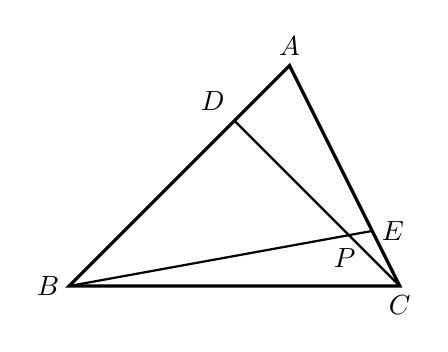
\begin{tikzpicture}[scale=0.7]
 \coordinate (A) at (4,4) node at (A) [above] {$A$}; % A(4,4)を設定,上に$A$
 \coordinate (B) at (0,0) node at (B) [left] {$B$}; % B(0,0)を設定,左に$B$
 \coordinate (C) at (6,0) node at (C) [below] {$C$}; % C(6,0)を設定,下に$C$

 \coordinate (D) at (3,3) node at (D) [above left] {$D$}; % D(3,3)を設定,左上に$D$
 \coordinate (E) at (5.5,1) node at (E) [right] {$E$};

 \draw [very thick] (A) -- (B) -- (C) -- cycle;
 \draw [thick] (C) -- (D);
 \draw [thick] (B) -- (E);

 \node at (5,0.5) {$P$};
\end{tikzpicture}
\end{minipage}


\dotfill


$\triangle ACD$と$\triangle ABE$を利用し、
それぞれにおいて
$\overrightarrow{\mathrm{AP}}$を$\vec{b},\vec{c}$で表す。


$\triangle ACD$において、
$CP:PD$を$s:(1-s)$とすると
$\overrightarrow{\mathrm{AP}}$は次のように表せる。
\begin{equation}
 \overrightarrow{\mathrm{AP}}
  =(1-s)\overrightarrow{\mathrm{AC}}+s\overrightarrow{\mathrm{AD}}
  = (1-s)\vec{c} + \frac{s}{3}\vec{b}
\end{equation}

$\triangle ABE$において、
$BP:PE$を$t:(1-t)$とすると
$\overrightarrow{\mathrm{AP}}$は次のように表せる。
\begin{equation}
 \overrightarrow{\mathrm{AP}}
  =(1-t)\overrightarrow{\mathrm{AB}}+t\overrightarrow{\mathrm{AE}}
  = (1-t)\vec{b} + \frac{3t}{4}\vec{c}
\end{equation}

この2つの
$\overrightarrow{\mathrm{AP}}$の表現より、
$\vec{b},\vec{c}$の係数が等しくなるように考えると
次の2つの式が得られる。
\begin{equation}
 \frac{s}{3} = 1-t
  ,\quad
  1-s = \frac{3t}{4}
\end{equation}

これより$s=\frac{1}{3} ,\; t=\frac{8}{9}$となるため、
$\overrightarrow{\mathrm{AP}}$は次のようになる。
\begin{equation}
 \overrightarrow{\mathrm{AP}}
  = \frac{1}{9}\vec{b} + \frac{2}{3}\vec{c}
\end{equation}


%%%%%%%%%%%%%%%%%%%%%%%%%%%%%%%%%%%%%%%%
\hrulefill

\begin{minipage}[c]{250pt}
 $\triangle \mathrm{OAB}$において、
 辺$\mathrm{OB}$の中点を$\mathrm{M}$、
 辺$\mathrm{AB}$を$1:2$に内分する点を$\mathrm{C}$、
 辺$\mathrm{OA}$を$2:3$に内分する点を$\mathrm{D}$、
 線分$\mathrm{CM}$と線分$\mathrm{BD}$の交点を$\mathrm{P}$とする。
 また、
 $\overrightarrow{\mathrm{OA}}=\vec{a}, \: \overrightarrow{\mathrm{OB}}=\vec{b}$とする。

 \begin{enumerate}
 \item $\overrightarrow{\mathrm{OP}}$を$\vec{a}, \: \vec{b}$を用いて表せ。
 \item 直線$\mathrm{OP}$と
       辺$\mathrm{AB}$の交点を$\mathrm{Q}$とするとき、
       $\mathrm{AQ:QB}$を求めよ。
 \end{enumerate}
\end{minipage}
%
\begin{minipage}[c]{200pt}
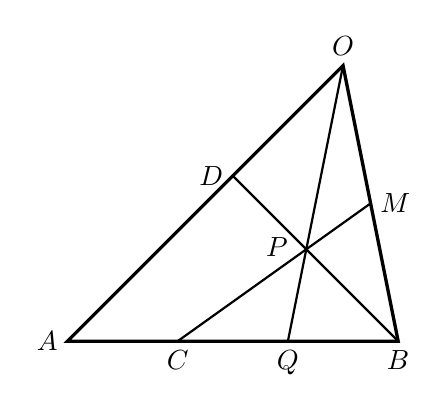
\begin{tikzpicture}[scale=0.7]
 \coordinate (O) at (5,5) node at (O) [above] {$O$}; % O(5,5)を設定,上に$O$
 \coordinate (A) at (0,0) node at (A) [left] {$A$}; % A(0,0)を設定,左に$A$
 \coordinate (B) at (6,0) node at (B) [below] {$B$}; % B(6,0)を設定,下に$B$

 \coordinate (C) at (2,0) node at (C) [below] {$C$}; % C(2,0)を設定,下に$C$
 \coordinate (D) at (3,3) node at (D) [left] {$D$}; % D(3,3)を設定,左に$D$
 \coordinate (M) at (5.5,2.5) node at (M) [right] {$M$};
 \coordinate (Q) at (4,0) node at (Q) [below] {$Q$}; % Q(4,0)を設定,下に$Q$

 \draw [very thick] (O) -- (A) -- (B) -- cycle;
 \draw [thick] (B) -- (D);
 \draw [thick] (O) -- (Q);
 \draw [thick] (C) -- (M);

 \node at (3.8,1.7) {$P$};
\end{tikzpicture}
\end{minipage}

\dotfill


\begin{enumerate}
 \item
      点$P$は線分$BD$の内分点である。
      $BP:PD = s : (1-s)$とすると、
      $\overrightarrow{\mathrm{OP}}$は次のように表せる。
      \begin{equation}
       \overrightarrow{\mathrm{OP}}
        = (1-s)\overrightarrow{\mathrm{OB}} +  s\overrightarrow{\mathrm{OD}}
        = (1-s)\vec{b} + \frac{2s}{5}\vec{a}
      \end{equation}

      点$P$は線分$CM$の内分点である。
      $CP:PM = t : (1-t)$とすると、
      $\overrightarrow{\mathrm{OP}}$は次のように表せる。
      \begin{equation}
       \overrightarrow{\mathrm{OP}}
        = (1-t)\overrightarrow{\mathrm{OC}} +  t\overrightarrow{\mathrm{OM}}
        = (1-t)(\vec{a}+\frac{1}{3}(\vec{b}-\vec{a})) + \frac{t}{2}\vec{b}
        = \frac{2(1-t)}{3}\vec{a} + \frac{2+t}{6}\vec{b}
      \end{equation}

      この2つの式の
      $\vec{a},\vec{b}$の係数から
      次の式を得る。
      \begin{equation}
       \frac{2s}{5} = \frac{2(1-t)}{3}
        ,\quad
        1-s = \frac{2+t}{6}
      \end{equation}

      これを解くと
      $s=\frac{5}{9} ,\; t=\frac{2}{3}$
      となり、
      $\overrightarrow{\mathrm{OP}}$は次のように求まる。
      \begin{equation}
       \overrightarrow{\mathrm{OP}}
        = \frac{2}{9}\vec{a} + \frac{4}{9}\vec{b}
      \end{equation}


 \item
      $AQ:QB = m:n$とすると、
      $\overrightarrow{\mathrm{OQ}}$は
      次のようになる。
      \begin{equation}
       \overrightarrow{\mathrm{OQ}}
        = \frac{n\vec{a}+m\vec{b}}{m+n}
      \end{equation}

      また、
      $\overrightarrow{\mathrm{OQ}}$は
      $\overrightarrow{\mathrm{OP}}$の定数倍であるので、
      $\overrightarrow{\mathrm{OQ}} = k\overrightarrow{\mathrm{OP}}$
      となる$k$が存在する。

      $\overrightarrow{\mathrm{OP}}$は次のような式に変形できる。
      \begin{equation}
       \overrightarrow{\mathrm{OP}}
        = \frac{2}{9}\vec{a} + \frac{4}{9}\vec{b}
        = \frac{6}{9}\left( \frac{2}{6}\vec{a} + \frac{4}{6}\vec{b} \right)
        = \frac{2}{3} \cdot \frac{\vec{a} + 2\vec{b}}{2+1}
      \end{equation}

      ここから、
      $\frac{3}{2}\overrightarrow{\mathrm{OP}}$は
      $AB$を$2:1$に内分する点を終点とするベクトルであることがわかる。

      点$Q$は$AB$の内分点であり、
      直線$OP$上の点である為、
      $\frac{3}{2}\overrightarrow{\mathrm{OP}}$の終点が$Q$ということとなる。

      よって、
      $AQ:QB=2:1$である。

\end{enumerate}



\hrulefill

\end{document}
